\section{HOSVD+GPR Surrogate Model for the ULB Hydrogen-Fuelled Flameless Furnace}
\label{sec:ulb}

\subsection{ULB hydrogen-fueled flameless furnace}
\label{sec:DATA_ULB}

This dataset comes from 2D CFD RANS of the ULB-modified stagnation-point reverse-flow combustor (SPRF) operating under flameless combustion conditions~\cite{giuntini2024continuously}. The domain is reduced to consider only the internal chamber of the burner. This choice was made to leave open the option of easily interpolating the data if necessary. The total number of available simulations is 175, but only 20 of them lie on a regular grid of operating conditions and are therefore suitable for an analysis with tensorial methods. This dataset is used to develop and validate the HOSVD+GPR reduced order model described in Section~\ref{sec:method_hosvd_gpr}.
The aforementioned grid is defined by three parameters: equivalence ratio $\phi$, hydrogen blending fraction in the fuel $H_2$, and operating pressure $p$:
\[
  \phi \in \{1.1,\,1.2,\,1.3,\,1.4,\,1.6\},
  \quad H_2 \in \{0.0,\,0.3\}\;\text{vol\%},
  \quad p \in \{1,\,2\}\;\text{atm}.
\]
These parameters are the ones that an operator can set before starting the combustion.

The data is arranged in a 5 dimensional tensor:
\[
  \mathcal{T} \;\in\; \mathbb{R}^{N_\phi \times N_{H_2} \times N_p \times N_{\mathrm{feat}} \times N_{\mathrm{cells}}},
\]
The analysis is performed solely on themorchemical variables, so temperature T and the 9 species $
\{N_2,\ NH_2,\ NO_2,\ H_2O,\ OH,\ O_2,\ H_2,\ NH_3,\ NO,\ T\}
$
indexed by $N_{\mathrm{feat}}$The 4 operating points with $\phi = 1.3$ are held out as the test set; the remaining 16 form the training set.
Figure~\ref{fig:ulb_data} shows an example of one data point for a given operating condition ($\phi$ = 1.2, $H_2$ = 0.3 vol\%, $p$ = 2 atm ):
\FloatBarrier
\begin{figure}[htbp]
    \centering
    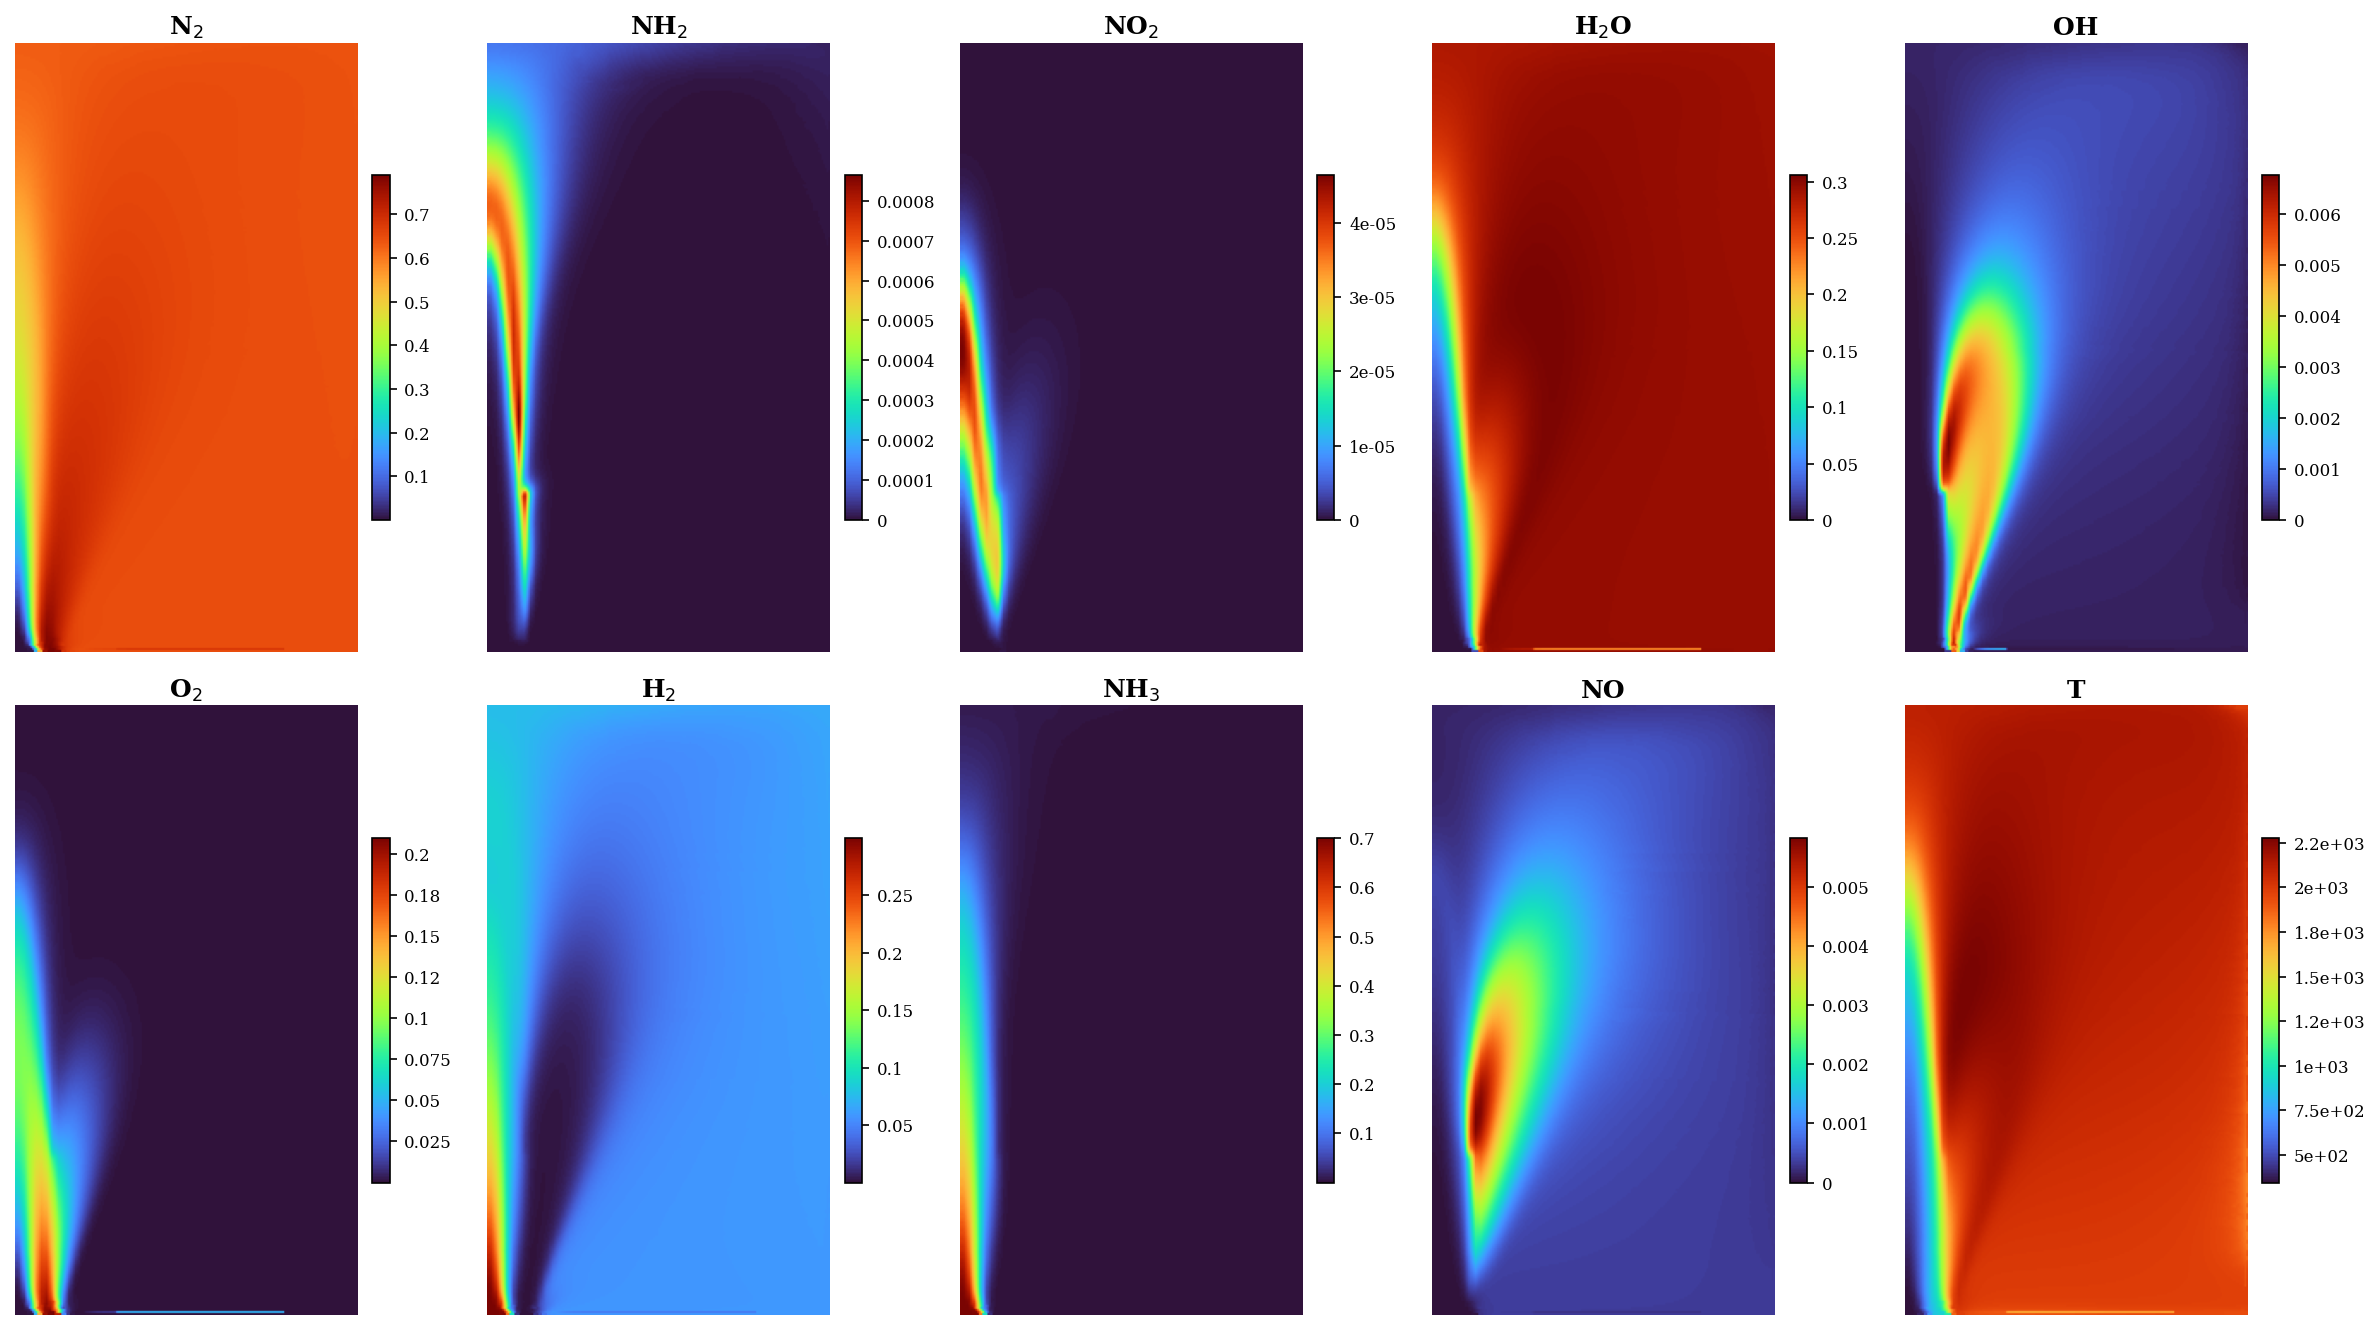
\includegraphics[width=0.95\textwidth]{../IMAGES/DATASETS/ulb_burner.png}
    \caption{Thermochemical variables of the ($\phi$ = 1.2, $H_2$ = 0.3 vol\%, $p$ = 2 atm) operating conditions point in the ULB-modified SPRF furnace.}
    \label{fig:ulb_data}
\end{figure}
\FloatBarrier

\subsection{Methods}
\label{sec:methods_ulb}

\subsubsection{HOSVD+GPR reduced order model for parametric interpolation}
\label{sec:method_hosvd_gpr}

The method is developed in the scope of surragate modeling. In particular, a crucial step towards the realization of fully working digital twins is the ability of leveraging high fidelity simulations to generate data for new operating conditions. In other words, the goal is that of beeing able to predict the behaviour of the system in unseen points of the operating condition space, so in practice the task is that of super resolution. Proper Orthogonal Decomposition (POD) combined with Gaussian Process Regression (GPR) has been succesfully employed in the past for this task~\cite{aversano2021digital}. The approach proposed here extends it to tensorial data by replacing the matrix SVD with High Order Singular Value Decomposition (HOSVD)~\cite{de2000multilinear}.

\paragraph*{Decomposition}

Given the 5-way data tensor $\mathcal{T} \in \mathbb{R}^{N_\phi \times N_{H_2} \times N_p \times N_{\mathrm{feat}} \times N_{\mathrm{cells}}}$ introduced in Section~\ref{sec:DATA_ULB}, HOSVD yields a multilinear decomposition
\[
  \mathcal{T} = \mathcal{G}
    \times_1 \mathbf{U}_\phi
    \times_2 \mathbf{U}_{H_2}
    \times_3 \mathbf{U}_p
    \times_4 \mathbf{U}_{\mathrm{feat}}
    \times_5 \mathbf{U}_{\mathrm{cells}},
\]
where $\mathcal{G}$ is a core tensor and each factor matrix $\mathbf{U}^{(n)}$ captures the variability along its respective dimension, obtained by truncated SVD of the $n$-mode unfolding of $\mathcal{T}$.

\paragraph*{Interpolation via GPR}

A 1D Gaussian Process Regressor~\cite{williams1995gaussian} is trained on the rows of $\mathbf{U}_\phi$, learning the mapping $\phi \mapsto \mathbf{U}_\phi$. The factor matrices $\mathbf{U}_{H_2}$, $\mathbf{U}_p$, $\mathbf{U}_{\mathrm{feat}}$, and $\mathbf{U}_{\mathrm{cells}}$ are held fixed at their training values, encoding the physical behaviour of the system along those axes without reparametrisation.

\paragraph*{Reconstruction}

For an unseen equivalence ratio $\phi^*$, the GPR predicts $\hat{\mathbf{U}}_\phi$ and the full thermochemical field is reconstructed as
\[
  \hat{\mathcal{T}} = \mathcal{G}
    \times_1 \hat{\mathbf{U}}_\phi
    \times_2 \mathbf{U}_{H_2}
    \times_3 \mathbf{U}_p
    \times_4 \mathbf{U}_{\mathrm{feat}}
    \times_5 \mathbf{U}_{\mathrm{c1ells}}.
\]
The full pipeline is summarised schematically in Figure~\ref{fig:ulb_pipeline}.

\FloatBarrier
\begin{figure}[htbp]
    \centering
    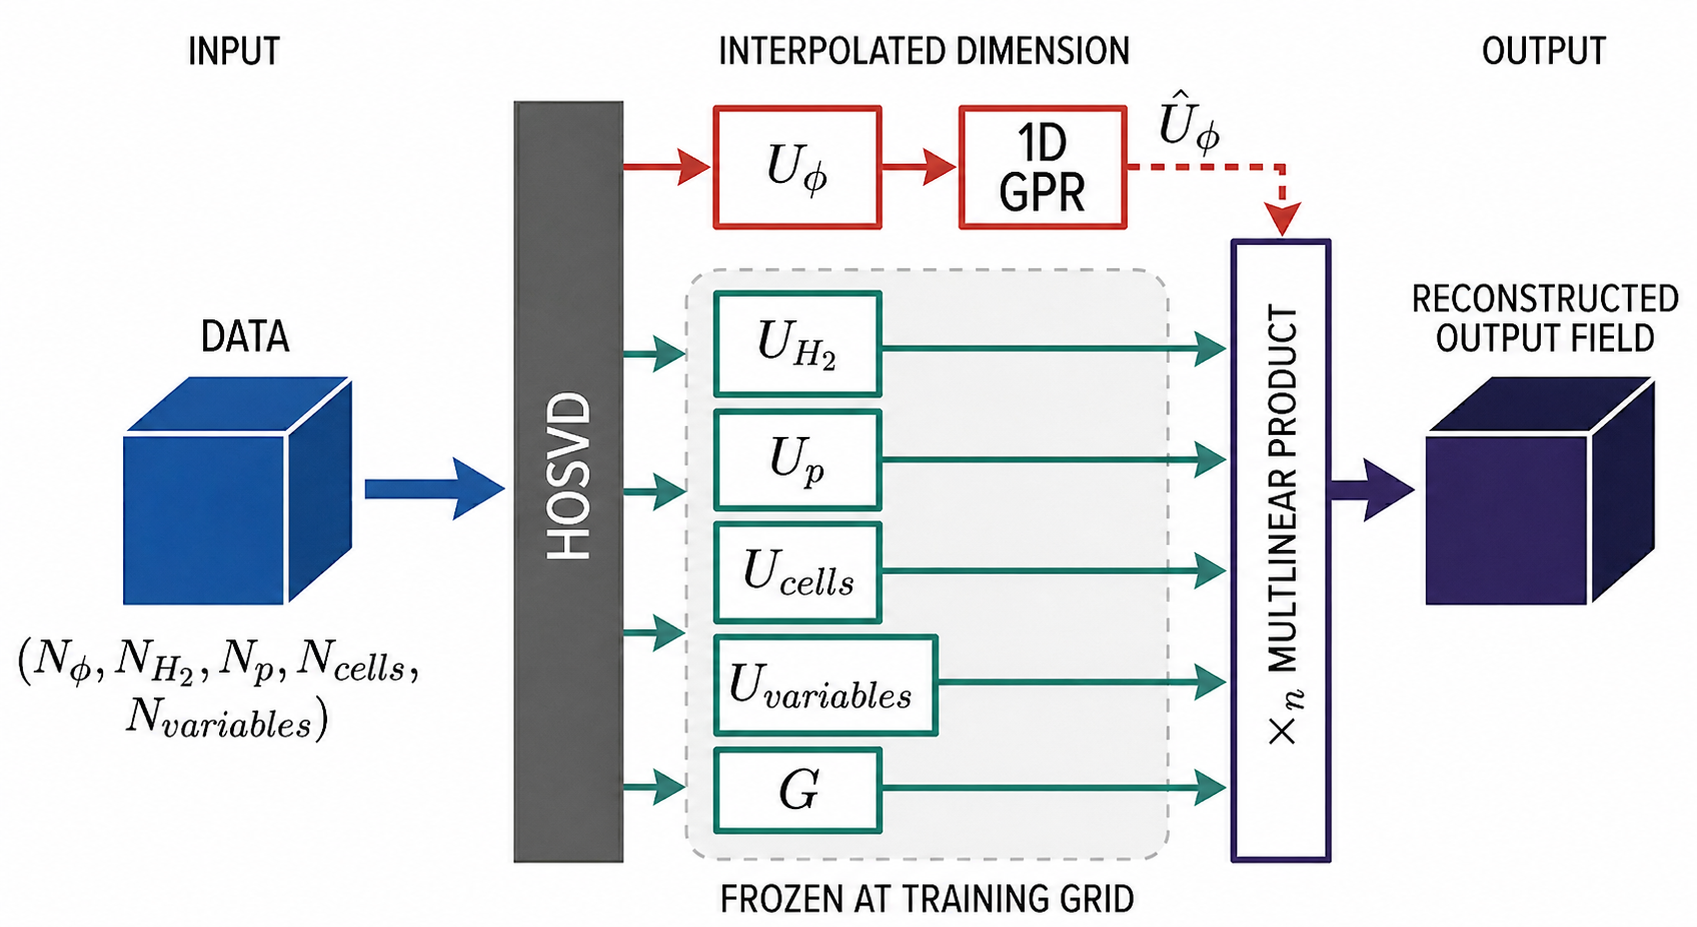
\includegraphics[width=0.80\textwidth]{../IMAGES/pipeline.png}
    \caption{Schematic of the HOSVD+GPR pipeline.}
    \label{fig:ulb_pipeline}
\end{figure}
\FloatBarrier

\subsection{Results and Discussion} \label{sec:results_ulb} Performance is evaluated on the 4 held-out operating points ($\phi = 1.3$, all $H_2$ and $p$ combinations) using the normalised root mean square error (NRMSE) with range normalisation, which makes the metric comparable across variables with very different magnitudes. The POD+GPR baseline is computed following~\cite{aversano2021digital}.
Figure~\ref{fig:ulb_temp_reconstruction} shows the temperature field reconstruction for one of the held-out conditions. The HOSVD+GPR prediction captures the spatial structure of the flame more accurately, with the largest discrepancies concentrated near the reaction zone where gradients are steepest.
\FloatBarrier
\begin{figure}[htbp]
\centering
\begin{minipage}[t]{0.54\textwidth}
    \centering
    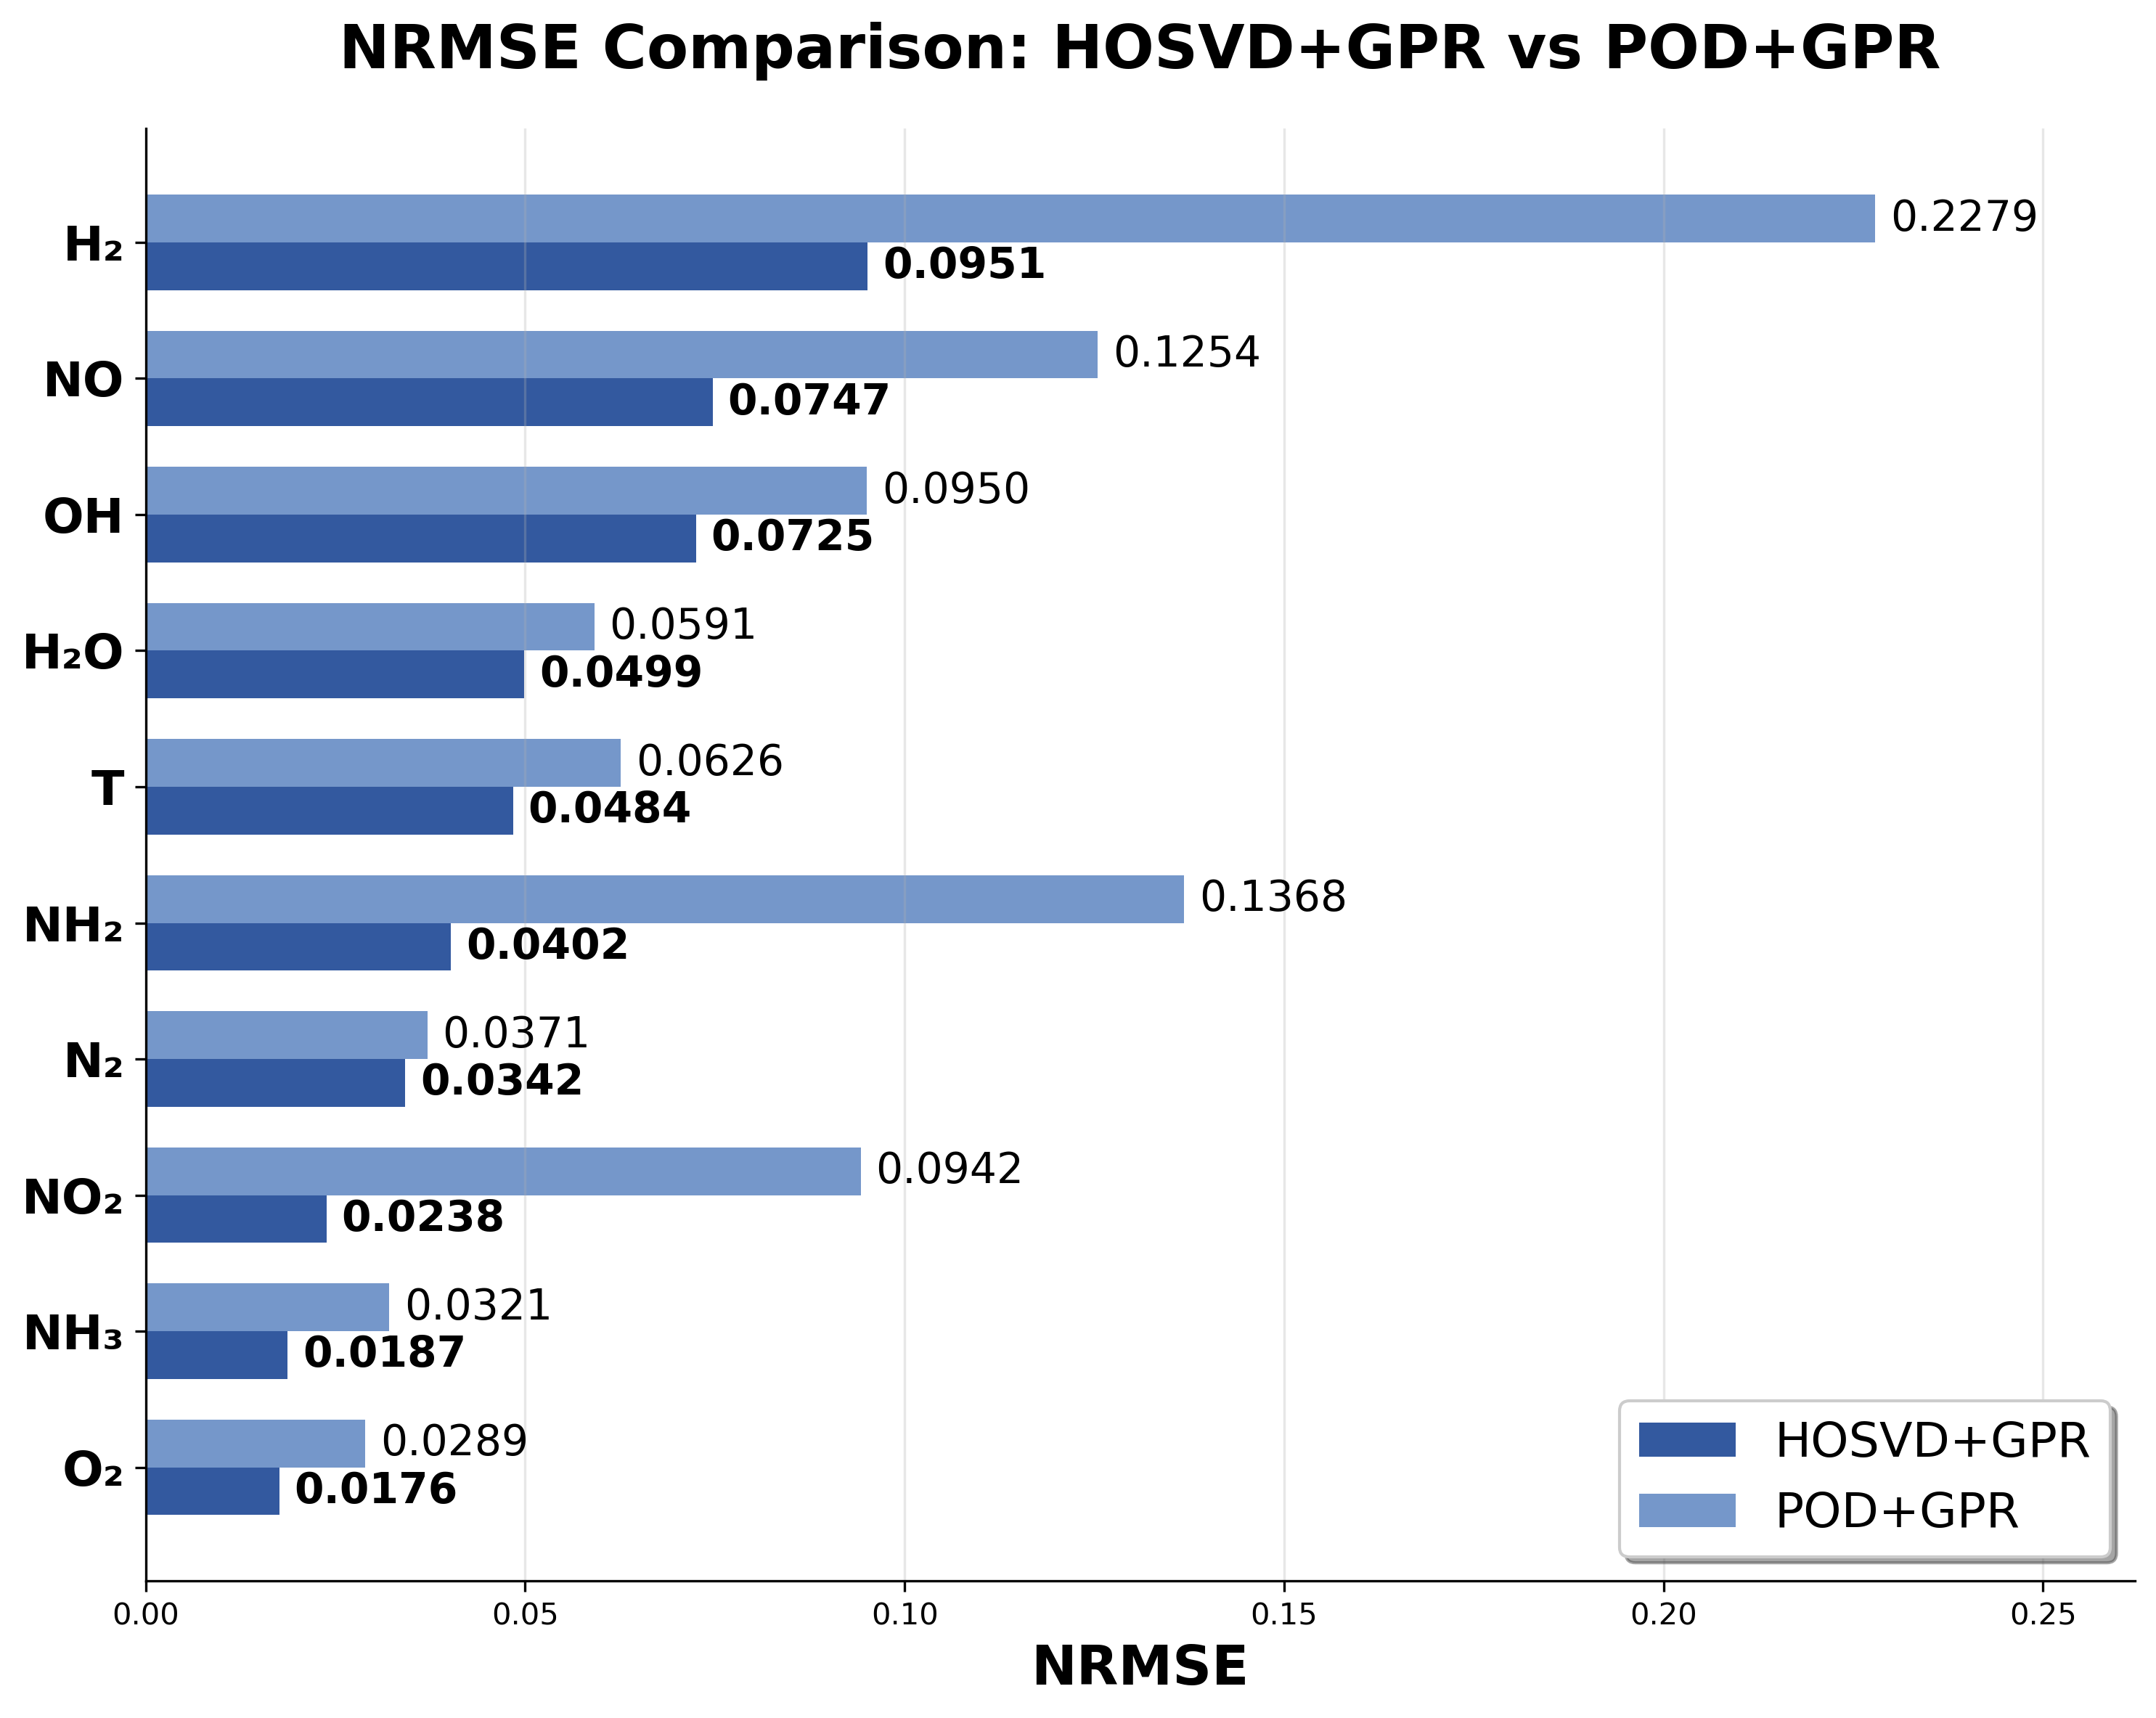
\includegraphics[width=\textwidth]{../IMAGES/horizontal_bar_comparison.png}
\end{minipage}
\hfill
\begin{minipage}[!t]{0.42\textwidth}
    \centering
    \scriptsize
    \begin{tabular}{lccc}
    \toprule
    Variable & HOSVD+GPR & POD+GPR & Improvement \\
    \midrule
    N$_2$   & 0.0342 & 0.0371 &  7.8\,\% \\
    NH$_2$  & 0.0402 & 0.1368 & 70.6\,\% \\
    NO$_2$  & 0.0238 & 0.0942 & 74.8\,\% \\
    H$_2$O  & 0.0499 & 0.0591 & 15.7\,\% \\
    OH      & 0.0725 & 0.0950 & 23.7\,\% \\
    O$_2$   & 0.0176 & 0.0289 & 39.2\,\% \\
    H$_2$   & 0.0951 & 0.2279 & 58.3\,\% \\
    NH$_3$  & 0.0187 & 0.0321 & 41.7\,\% \\
    NO      & 0.0747 & 0.1254 & 40.4\,\% \\
    $T$     & 0.0484 & 0.0626 & 22.6\,\% \\
    \bottomrule
    \end{tabular}
\end{minipage}
\caption{NRMSE comparison between HOSVD+GPR and POD+GPR across all predicted
variables. The bar chart (left) and table (right) both show that HOSVD+GPR
consistently outperforms POD+GPR, with the largest improvements observed for
NH$_2$ (70.6\,\%), NO$_2$ (74.8\,\%), and H$_2$ (58.3\,\%).}
\label{fig:nrmse_comparison}
\end{figure}
\FloatBarrier

\FloatBarrier
\begin{figure}[htbp]
    \centering
    \caption{Temperature field reconstruction for a held-out condition ($\phi = 1.3$). Left: CFD reference. Centre: HOSVD+GPR (NRMSE\,=\,0.0484). Right: POD+GPR (NRMSE\,=\,0.0626). [Add figure when available.]}
    \label{fig:ulb_temp_reconstruction}
\end{figure}
\FloatBarrier

\subsubsection*{Discussion}

